\documentclass[7x9]{times}

% use MIT book class


\title{Penetration Testing and Ethical Hacking}
\author{Many authors}
%\institude{Nanjing University, China}
\date{\today}
\edition{2019 Edition}



%% For multiple indices:
%\usepackage{multind}
%\makeindex{topics}
%\makeindex{authors}

\def\taupav{\tau_{\mathrm{Pav}}}

\newbox\oiintbox
\setbox\oiintbox=\hbox{$\lower2pt\hbox{\huge$\displaystyle\circ$}
	\hskip-13pt\displaystyle\int\hskip-7pt\int_{S}\ $}
\def\oiint{\copy\oiintbox}

\def\boldnabla{\hbox{\boldmath$\displaystyle\nabla$}}

\nocropmarks

\usepackage{multind}
\makeindex{topics}
\makeindex{authors}

\usepackage{listings}
\lstloadlanguages{bash,Python}

\DeclareGraphicsExtensions{.eps,.pdf,.png,.jpg}

\usepackage[caption=false,font=footnotesize]{subfig}

\begin{document}

%[frontmatter] turns off chapter numbering and uses roman
% numerals for
%page numbers; [mainmatter] turns on chapter numbering,
% resets page
%numbering and uses arabic numerals for page numbers;
% [appendix]
%resets chapter numbering, uses letters for chapter numbers
% and
%doesn't fiddle with page numbering; [backmatter] turns off
% chapter
%numbering and doesn't fiddle with page numbering.

\titlepage

\begin{copyrightpage}

  \copyright\ 2019 Center for Cybersecurity and Cybersecurity Malaysia
	
	All rights reserved. No part of this book may be reproduced in
        any form or by any electronic or mechanical means (including
        photocopying, recording, or information storage and retrieval)
        without permission in writing from the publisher.
	
	
	This book was set in Minion Pro and Myriad Pro by the author.
	
	Printed and bound in the United States of America.
	
	MIT License. This work is licensed under a Creative Commons Attribution 
	4.0 International License.
	
	Penetration Testing and Ethical Hacking/ .\\
	\hspace*{6pt} p. cm.
	
	Includes bibliographical references and index.\\ ISBN ????
        \vfill
	
	10\ 9\ 8\ 7\ 6\ 5\ 4\ 3\ 2\ 1\
	
\end{copyrightpage}

\tableofcontents
\listoffigures
\listoftables

\begin{contributors}[twocolumn]
	
	\contrib 
	Mohd Zamri Murah\\
	Center for Cybersecurity\\
	Universiti Kebangsaan Malaysia
	
	\contrib 
	Professor Andrei Linde\\
	Department of Physics\\
	Stanford University\\
	Stanford, CA, USA
\end{contributors}


\begin{preface}

ALhamduiLlah. This book is based on lecture notes for
\textit{TX6244:Ethical Hacking and Penetration Testing}, a course
offered by Center for Cybersecurity(UKM) since 2014. This course is
jointly developed by Center for Cybersecurity(UKM) and Cybersecurity
Malaysia(CSM).

We hope this book will provide a good overview for students into the
field of penetration testing and ethical hacking. We also hope these
materials will encourage students to further explore this exciting
field.

We try hard to be current up to 2019. However, this is a tall order
with the amount of information available on the Internet. As always,
please inform of any errors or omissions to \url{zamri@ukm.edu.my}.

The book source code is available on
\url{github.com/mohdzamrimurah/bukusiber}, and we welcome
collaboration from all users.



\end{preface}

\chapter{Introduction to Ethical Hacking}

\paragraph{Cyber attacks} have increasing common in the past
years. Many of these attack targeted business entities,
government websites, financial institutions, social network
sites, power utilities, education sites and other sites.
These attack could cause financial lost, data breach, lost
of consumer confidence, and other risks. Because of the
increase frequency and the severity of the cyber attacks,
many organizations begin to take proactive measure to assess
their own network security status. One of these proactive
step is penetration testing.

Penetration testing, or ethical hacking, is a process to
assess the security level of an organization. It consists of
structure steps on how to hack or to break into the
organization network, websites or it infrastructure by
simulating external cyber attacks on the organization. The
main purpose of a penetration testing is to discover
securities issues that could be exploited by cyber hackers
and to offer counter measures to these risks.

\section{Cyber attacks}

\paragraph{18/1/2019} A collection containing more than 87
gigabytes of personal information was leaked online. The
data dump had 772,904,991 email addresses, and 21,222,975
passwords. Data breaches continue to happen as companies
collect data on millions of people and fail to protect them
properly.  Marriott loss personal information belonging to
383 millions guests, Yahoo data belonging to 3 billions
accounts were stolen. About 147.7 millions Social Security
numbers taken in the Equifax data breach.

% https://www.zdnet.com/article/
% singapore-suffers-most-serious-data-breach-affecting-1-5m-
% healthcare-patients-including-prime/

\paragraph{In Singapore}, 1.5 millions patients of
SingHealth had been accessed and copied. The stolen data
included name, national identification number, address,
gender, race, and date of birth. Also, outpatient medical
data of some 160,000 patients were compromised. Hackers had
gained control through breaching a front-end workstation,
from which they then were able to obtain privileged account
credentials to gain access to SingHealth's database.
Cybersecurity vendors have warned that the compromised data
may find its way on the Dark Web.



\section{Categories of a Pen Test}

It is easier if we could category the type of Pen Test available. Typically, 
a Pen Test could be done on 5 categories;
\begin{enumerate}
    \item network
    \item web apps
    \item mobile apps
    \item wireless
    \item desktop and server
\end{enumerate}

By understanding that there are different type of pen test,
we could then learn how to do a pen test for each particular
category. For instance, in doing a pen test for a web site,
we normally uses exploitation tools such as \url{Netsparker}
and \url{Acunetix}. These tools will discover and enumerate
vulnerabilities on the web site. On the other hand, if we
are doing a pen test on a network, we would use \url{nmap}
or \url{Nessus} to discover vulnerabilities on the network.
If we are testing wireless network, we could use
\url{Wireshark} to capture the wireless traffic.

It is important to realize the type of a pen test we are
doing, and what kind of tools available to do the pen test.
This is an important first step in a pen test.


\chapter{Tools and Software}


\paragraph{Tools and Software} This chapter contains
information about basic essential tools and software for
penetration testing. Familiarity of these tools would make
it easier to conduct penetration testing.


\section{Linux}

Linux\cite{sobell2015practical,barrett2016linux} is an
operating system for computer, much like Window 10 or Mac
OSX. It is based on Unix. Linux was first developed in 1991
by Linus Torvalds, a Finnish graduate student. Today, it is
being develops and maintains by a group of software
developers head by Linus Torvalds. It is widely uses in
large technology companies like Google, Facebook, and
Amazon. Linux is widely used as business servers for
businesses daily operation. It is estimated that 70\% of web
servers use Linux, with 30\% of web servers using
Window-based.

Linux is open source and free for everybody to use and to
modify. The open source creative license make it possible
for any person or organization to modify Linux to fit their
needs. For example, Chinese government produce their own
amended version of Linux for the Chinese
market(\url{http://www.kylinos.com.cn/}). Similarly, many
organizations such as NSA, Google(\url{gLinux}), Amazon have
customized Linux for their need. Figure~\ref{fig:ubuntu}
shows a Linux Ubuntu desktop.

There are many Linux distributions such as Ubuntu, SuSE,
Debian and Red Hat. Red Hat(Linux) is widely used as
business servers, Ubuntu is by customer desktop and Debian
is commonly uses by software developers. A Linux
distribution is a Linux operating system with other useful
software such as text editor, pdf viewer, browser, music
player and image processing. A Linux distribution is similar
to a PC with Window 10, Microsoft Office software and other
familiar software applications.

\index{topics}{Linux}
\index{topics}{Kali Linux}

%\begin{center}
%	\begin{figure}[]
%		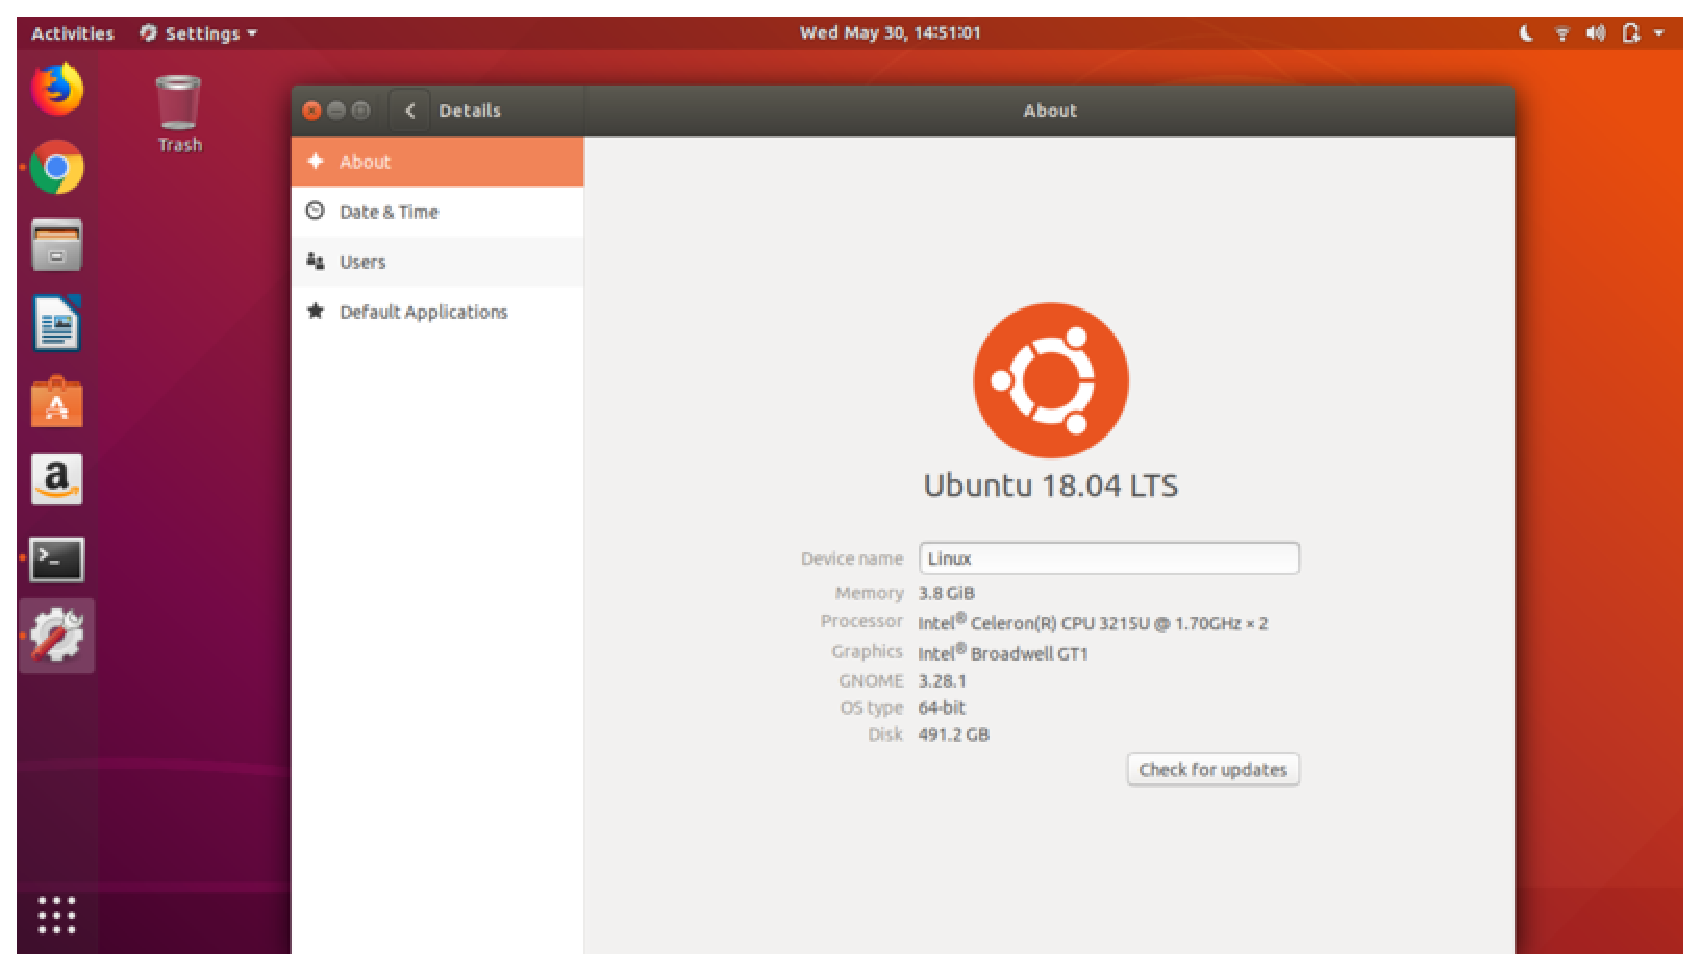
\includegraphics[scale=.5]{Ubuntu-18.04.eps}
%		\caption{Linux Ubuntu version 18.04 desktop.}
%		\label{fig:ubuntu}
%	\end{figure}
%\end{center}

\paragraph{Kali Linux}is a Linux distribution for
penetration testers. It consists of many widely used tools
for pentest. This distribution make it easy to use common
tools in a pentest. There are about 200+ tools in Kali Linux
for various stages of a pentest. Figure~\ref{fig:kali} show
a Kali Linux distributions with tools for penetration
testing.

%\begin{center}
%	\begin{figure}[]
%		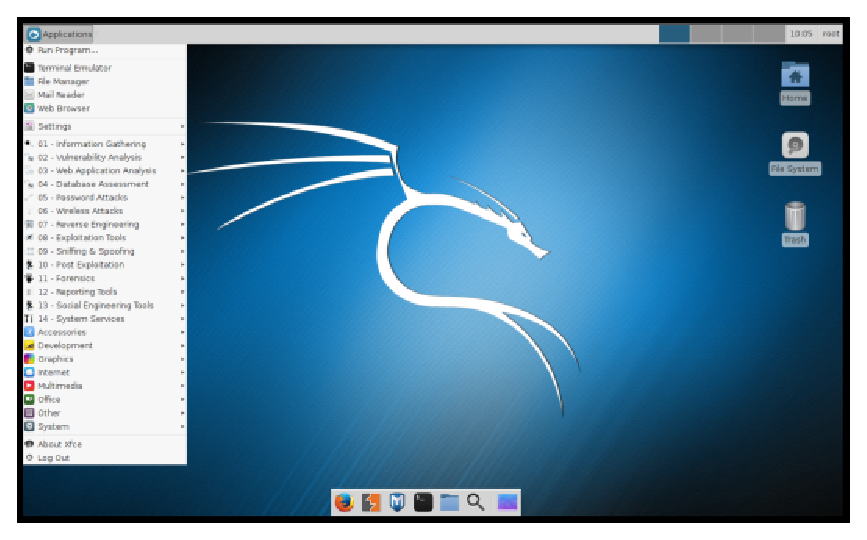
\includegraphics[scale=.5]{kali-linux.eps}
%		\caption{Kali Linux. A Linux distribution for pen testers.}
%		\label{fig:kali}
%	\end{figure}
%\end{center}

\begin{figure*}[!t]
\centering
\subfloat[Kali 
Linux]{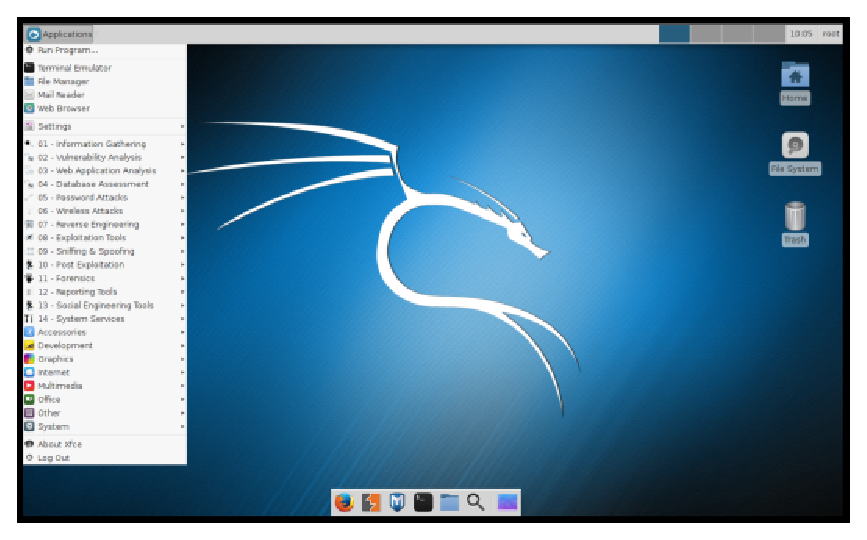
\includegraphics[width=.45\textwidth]{kali-linux}%
\label{fig:kali}}
\hfil
\subfloat[Ubuntu 
Linux]{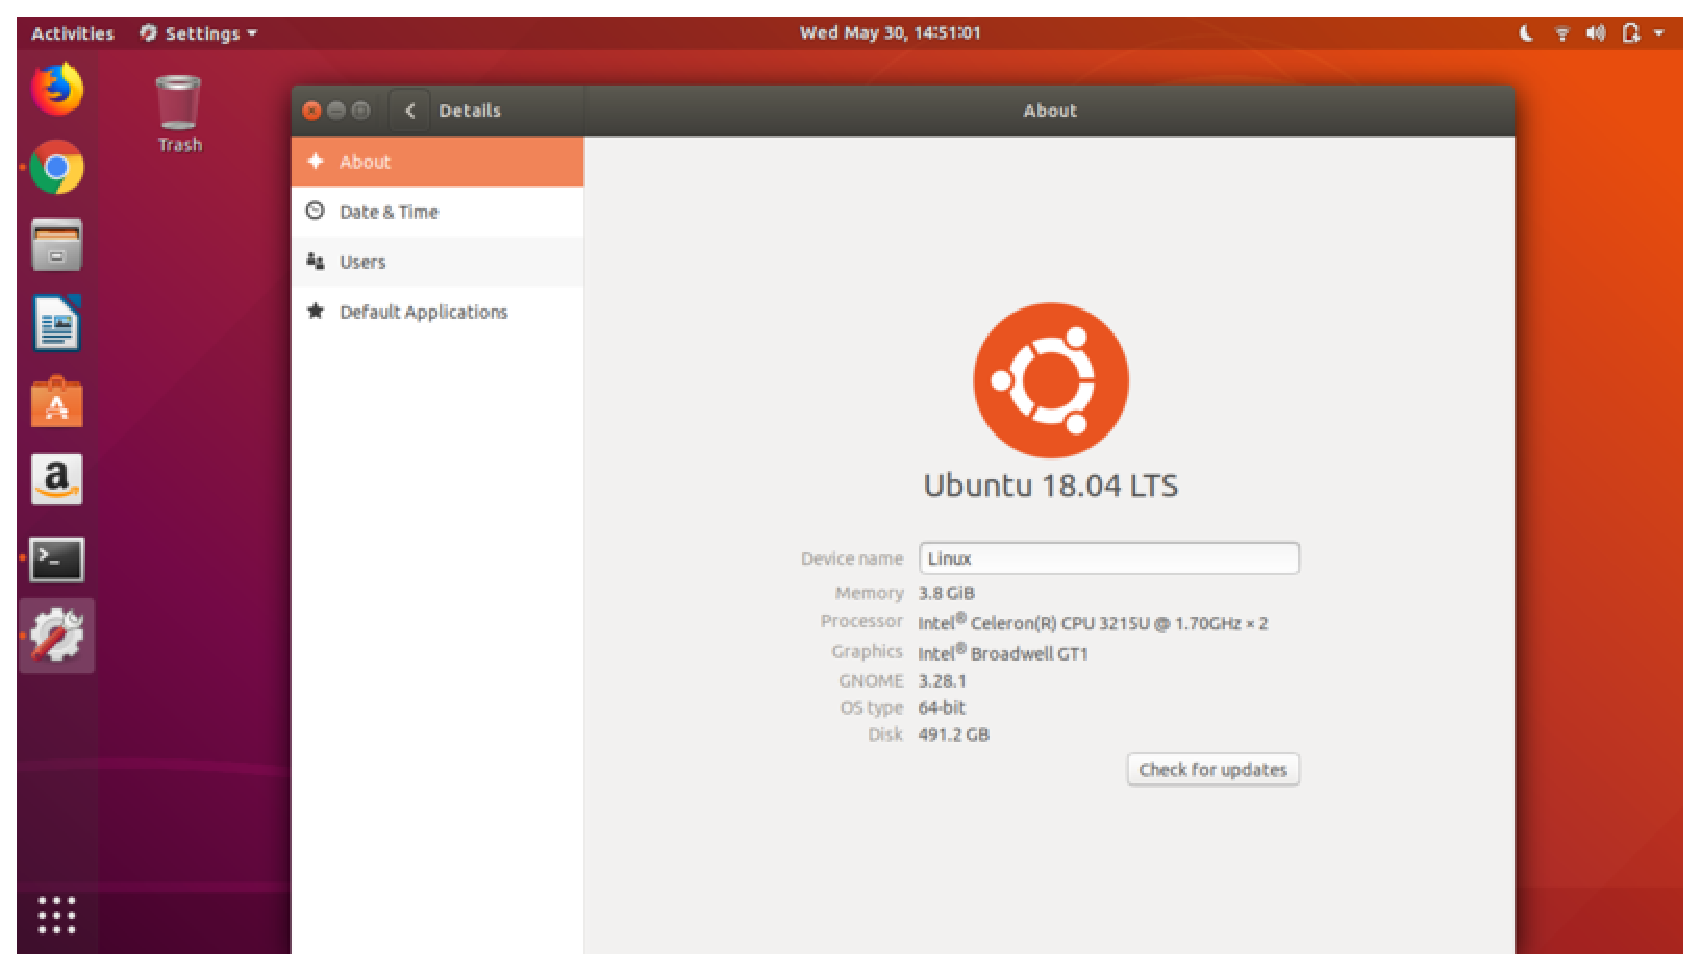
\includegraphics[width=.45\textwidth]{Ubuntu-18.04.eps}%
\label{fig:ubuntu}}
\caption{Example of Linux distributions.}
\label{fig:linux}
\end{figure*}

There exist various approach in installing and using Linux.
One of the easiest is to install Kali Linux on a standalone
machine. Another is to install Kali Linux as a dual boot
system together with Window 10/7. Another approach is to
install Kali Linux on a virtual machine such as VirtualBox
or VMware. Another is using docker. And, for more advance
user, you can run Kali Linux on the cloud, without
installing anything on your computer. Please google for more
information if you are interested in installing Kali Linux
as your pen test platform.

\index{topics}{docker}


One widely used Linux derivative is Android, an operating
system used in mobile phone. It is estimated that Android
has a market share of about 70\% for mobile phone and 30\%
for iOS.



\section{git}

\paragraph{git}\cite{loeliger2012} is a source code
management tool. \url{github.com} is a git repository, where
software developers share their software source codes in the
Internet. \url{Github.com} host many open source pen test
tools projects such as \url{metasploit} and \url{nmap}. A
pen tester can clone the repository and install the software
on his machine. With this approach, the pen tester can
always use the latest version of the software.

A pen tester need to clone the repository from
\url{github.com}. An example for such action is given below
for cloning \url{nmap} repository. Figure~\ref{fig:github}
show a sample repository at \url{github.com}.


\verb|git clone https://github.com/nmap/nmap.git|

% https://www.online-convert.com/
% take screen shot in png, convert to eps

%\begin{center}
%	\begin{figure}[ht]
%		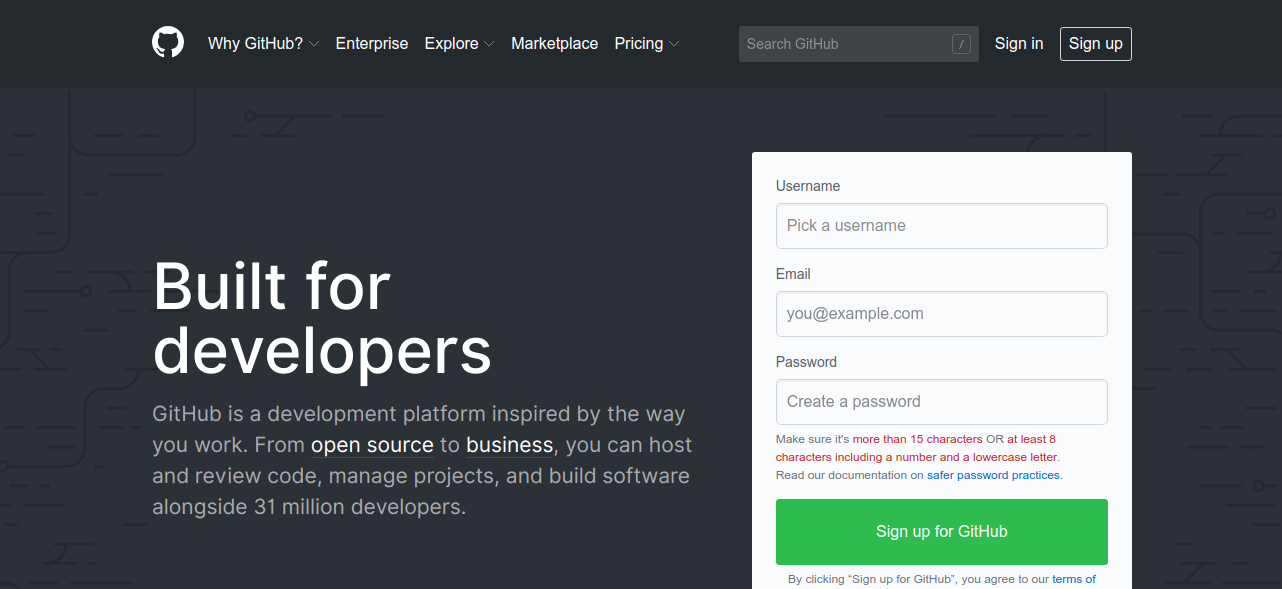
\includegraphics[width=.50\textwidth]{github.eps}
%		\caption{github.com}
%	\end{figure}
%\end{center}

\begin{figure}
\centering
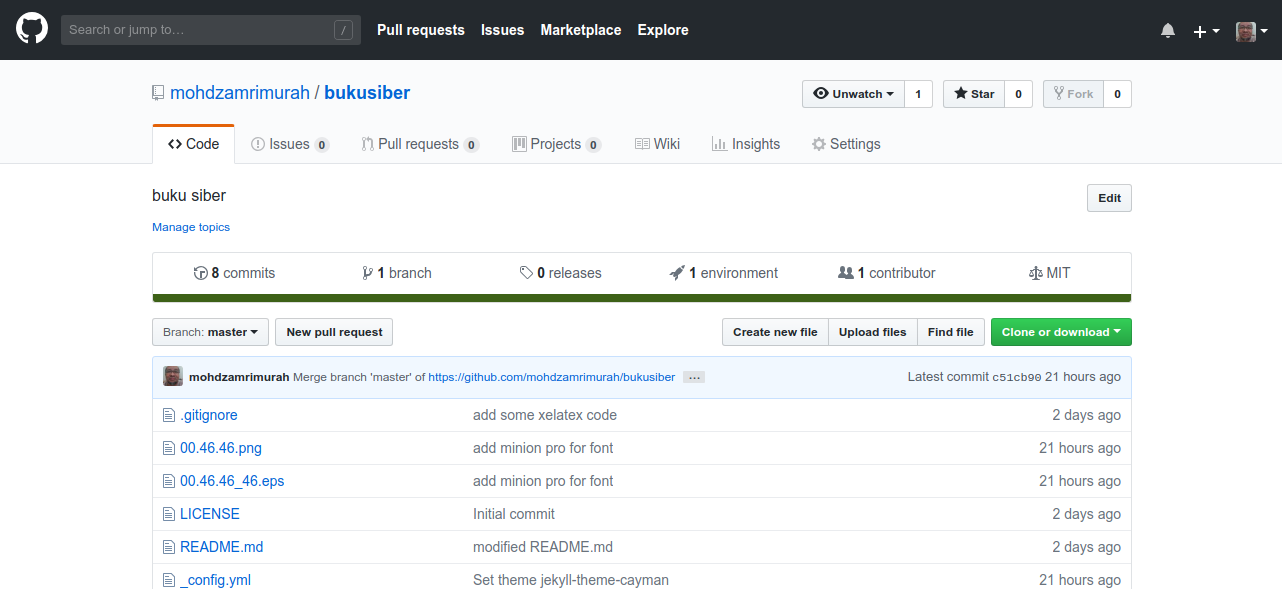
\includegraphics[width=.75\textwidth]{github-ui}
\caption{Source code repository at github.com}
\label{fig:github}
\end{figure}

\index{topics}{git} \index{authors}{Loeliger, Jon}

\section{Python}

\paragraph{Python}\cite{van2007python}\cite{lutz2013learning}
\cite{lutz2010programming} is a general-purpose, high-level 
programming language whose design philosophy emphasizes 
code readability. Currently, it is widely used in data 
science, deep learning and web development and software 
development. It has been used to develop tools for pen 
tests.  There are many pen test tools written in Python, 
hosted at \url{github.com}. An example is \url{Sublist3r}, 
a tool for network scanning and reconnaissance 
\index{topics}{Sublist3r}

\index{topics}{Python}
\index{authors}{Lutz, Mark}

Many processes in a pen test can be automated using Python.
We could develop new tools for pen tests, automated the
process and discovered new vulnerabilities.


%\section{Raspberry Pi}
%
%\paragraph{Raspberry Pi} is a small single-board computer. It can be used 

\section{Cybersecurity News}

\section{Web resources}

There exist tons of materials related to pen-test online. It
is best to adopt a life long attitude toward pen test where
one try to always update oneself with the latest info about
pen test. These are some of useful websites;
\begin{enumerate}
\item \url{https://github.com/enaqx/awesome-pentest}
\item \url{https://github.com/paralax/Awesome-Pentest-1}
\item \url{https://github.com/coreb1t/awesome-pentest-cheat-sheets}
\item \url{https://pen-testing.sans.org/}
\end{enumerate}

Another useful site is \url{https://www.quora.com/}. It is
question and answer website. This website contain some of
the latest info about a pen test.



\section{Cybersecurity Accreditation}

There are many industry-based certificates that a pen tester
could pursue to enhance marketability and to increase
knowledge. One of the certification is GPEN (GIAC
Penetration Tester)\footnote{
    \url{https://pen-testing.sans.org/certification/gpen}},
offered by SANS Institute. Another is OSCP (Offensive
Security Certified Pen Tester)\footnote{
\url{https://www.offensive-security.com/}}.  Another widely
accepted certification is CEH (Certified Ethical Hacking) by
EC-Council\footnote{\url{https://www.eccouncil.org/}}.


\section{Virtual Machine}

\paragraph{Virtualization} allow you to build a virtual lab 
for practice and simulation on your own desktop or note 
book. This require a desktop or notebook with a bit high 
requirement.

You can use
VMware\footnote{\url{https://my.vmware.com}}
 as your virtualization software. Using VMware, we could 
install Kali Linux as a virtual machine on a Window 10 
machine. This is the easiest way to run multiple OS on a 
single machine.

There are Kali Linux virtual machine images from the
Internet
\footnote{\url{https://www.offensive-security.com/}}.
 Download this and install Kali Linux on your
machine as a virtual machine.

Another approach is using docker or kubenetes. Yet another
option is running Kali Linux from the cloud. There are many
options for you to try to build your own penetration testing
environment.


\section{Summary}

For a basic skill, a pen tester need to be familiar with
Linux, especially Kali Linux. He also need to know \url{git}
and \url{github.com} for pen test tools repository. For
advance pen test, he could learn Python for automation and
advance exploit.

In summary, pen test is a wide field and there are almost unlimited information
in the Internet. 
\begin{center}
	\begin{figure}[ht]
		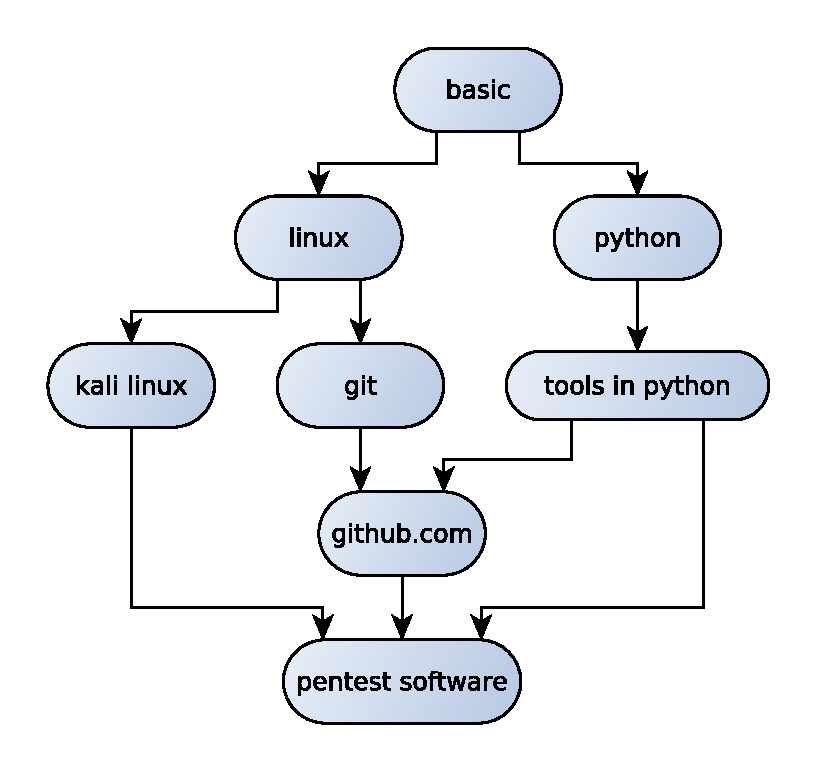
\includegraphics[scale=.75]{tools}
		\caption{Basic tools for pen testers.}
	\end{figure}
\end{center}

\begin{table}[]
    \begin{tabular}{|c|l|c|}
        \hline 
        Tool & Use &  \\ 
        \hline 
        Linux & operating system &  \\ 
        \hline 
        git & software repository &  \\ 
        \hline 
        Python & Programming language. advance pen test &  \\ 
        \hline 
    \end{tabular}
    \caption{Summary of common tools}
    \label{tab:tools}
\end{table}



\chapternotes
 

\chapter{Network Basic}

% based on SANS401

\paragraph{Network} is an important component in an 
organization. This is an introduction to the core concepts 
in computer networks and protocols.

\section{Network}

\paragraph{LAN} is is a computer network that interconnects
computers within a limited area such as a residence, school,
laboratory, university campus or office building. Ethernet
and Wi-Fi are the two most common technologies in use for
local area networks. Network topology describes the layout
of interconnections between devices and network segments.
The Internet Protocol Suite (TCP/IP) has prevailed as a
standard of choice for networking protocol.

\index{topics}{TCP/IP}

Users of LAN can pose threats to the networks. Unsuspected
users may install malicious software that spread through the
network. Users could also unknowingly install botnets, 
viruses, 
malware and other vulnerabilities.

\paragraph{Internet} is a network that connect many LANs,
WANs and other networks the world largest global network. A
topology describes how the network is wired together. There
are many types of topology as shown in
Figure~\ref{fig:topology}; bus, ring and star. The star
topology is widely used in a LAN. All nodes in this topology
are connected directly to a central device, such as a hub or
switch. A hub or a switch will control the networking
between the nodes.

\index{topics}{topology}
\paragraph{Hub} repeat the data that it receives on one port
to its other ports. A bridge is used to connect two segments
of a network. A switch combines the functionality of a hub
and a bridge into a single device. Sniffing becomes very
ineffective with switches. Routers interconnect logical
networks. A switch or a bridge connects physical segments
that reside on the same logical network. A router makes
decisions where to direct data that passes through it. A
router drops traffic if it does not know where to send it. A
switch or a bridge transmit traffic to unknown destinations.

\index{topics}{hub}


%\begin{figure}[ht]
%    \caption{Topology for a network}
%    \label{fig:topology}
%    \includegraphics{topology.jpg}
%\end{figure}

\begin{figure}[ht]
    \centering
    \subfloat[Types of 
    topology]{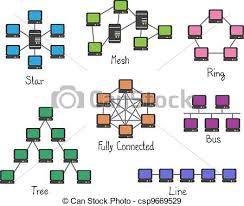
\includegraphics[width=.45\textwidth]{topo1}%
        \label{fig:topo1}}
    \hfil
    \subfloat[Ring 
    topology]{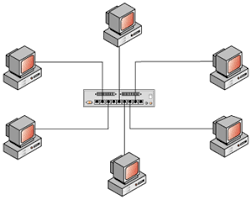
\includegraphics[width=.4\textwidth]{topo2}%
        \label{fig:topo2}}
    \hfil
    \subfloat[Combination of two 
    network]{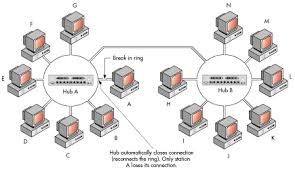
\includegraphics[width=.4\textwidth]{topo3}%
    \label{fig:topo3}}
    \caption{Topology for a network}
    \label{fig:topology}
\end{figure}

\paragraph{A virtual LAN (VLAN)} allows you to segment users
into different networks based on function or access
required. VLAN can limit the access or visibility by placing
the users on separate segments(Figure~\ref{fig:vlan1}). 
Network Access Control (NAC)
can be used to limit infected hosts from infecting other
nodes in the networks. If a single host becomes infected, it
can prevented from connecting to critical networks through
NAC and stopped from spreading to a large number of hosts
through VLANs. \index{topics}{VLAN}

\begin{figure}
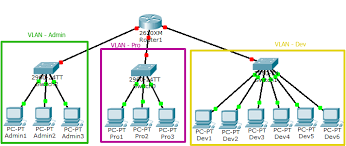
\includegraphics{vlan1.png}
\label{fig:vlan1}
\caption{VLAN}
\end{figure}

\begin{figure}
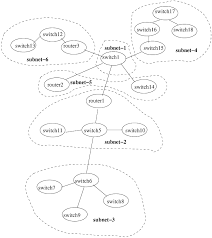
\includegraphics{vlan2.png}
\label{fig:vlan2}
\caption{VLAN}
\end{figure}

\section{Network Segment}

Typically an organization network is separated into 2 basic
categories; public and private. A public network is a
network that can be accessed form the Internet, and have
access to Internet. This network include an e-mails server,
web servers and DNS servers. A private network is a network
that could not be access from the Internet by normal users.
The information in the private network needs to be protected
from unauthorized users and cyber attacks. Example of a 
private network is database servers and organization 
information systems.Grouping similar resources together 
will allow us to better 
protect the networks.

\paragraph{Firewall} is one of the most fundamental ways of
protecting our systems from an external attack. It can be
used to control access or restrict traffic in the networks.
Basically, a firewall should grant access to Web, mails and
DNS traffic. The firewall should block any traffic to the
private networks.

\paragraph{Defense-In-Depth} is a security approach where
multiple layers of protection are used to protect the
networks. For example, in a network, we could use a firewall
to filter network data flow as one layer of protection, a
switch to route the traffic as another layer, and an IDS to
detection intrusion as another layer. Not relying on a
single later of security to protect against attacks is the
fundamental principle of defense-in-depth.
\index{topics}{defense-in-depth}
 


\section{Network concepts}

\paragraph{A network protocol} is basically how computers 
communicate with each other. This is how a host 
communicate with a server. The protocol make sure that each 
computer understand each other. Two computers need to use 
the same network protocol to be able to communicate with 
each other.

\paragraph{The OSI model} is one of the network protocol.
It consist of seven layers; physical, data link, network,
transport, session, presentation and application. The TCP/IP
model have four layers; network, Internet, transport and
application. Both models can be mapped into each other;
network (physical, data link), Internet(network), 
transport(transport), application(session, presentation, 
application)(Figure~\ref{fig:iso1},~\ref{fig:iso2}). 
\index{topics}{OSI 
model}

\begin{figure}
    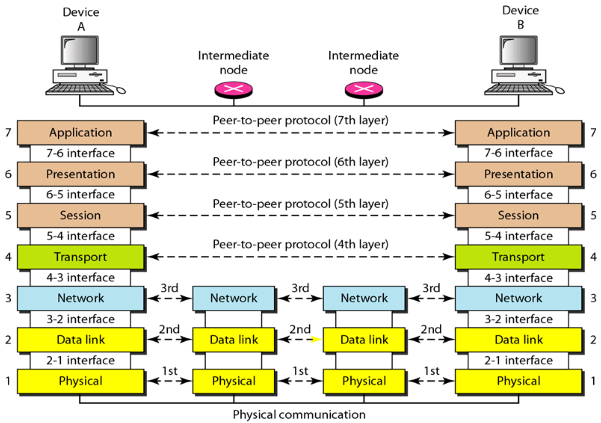
\includegraphics[]{GOySTAD}
    \caption{ISO model}
    \label{fig:iso1}
\end{figure}


\begin{figure}
    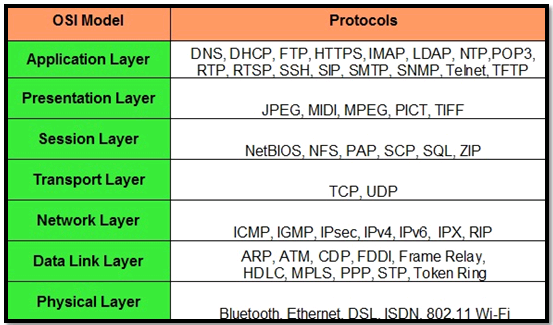
\includegraphics[width=.75\textwidth]{2Xd2IXV}
    \caption{ISO model}
    \label{fig:iso2}
\end{figure}

Each layers of the model is independent. This is a security 
issue. Layer independence makes it easier and faster to
maintain network, but pose a security issue.

\paragraph{lP(Internet Protocol)} is the basis for
communication on the internet. IP focused on getting packets
from point A to point B as efficiently as possible. IP 
protocol defined IP addressing scheme that uniquely 
identify a host and rules to route data between hosts. The 
IP data packet is shown in Figure~\ref{fig:packet}.
\index{topics}{IP protocol}

\begin{figure}
    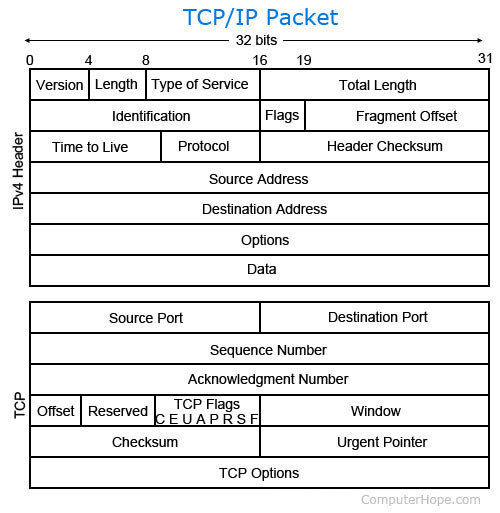
\includegraphics{packet}
    \caption{IP packet}
    \label{fig:packet}
\end{figure}

\section{IP address}

Each node in a network is identified by a unique IP address.
Part of the IP address is the network address. IP addresses
are denoted as four numbers separated by periods. Netmask
determines what portion of the address identifies the
network address. IP addresses are divided into 3 categories;
class A are allocated in the range of $1.0.0.0$ through
$127.255.255.255$ with subnet of $255.0.0.0$, Class B
networks are allocated in the range of $128.0.0.0$ through
$191.255.255.255$ with subnet of $255.255.0.0$, Class C
networks are allocated in the range of $192.0.0.0$ through
$223.255.255.255$ with subnet of $255.255.255.0$. However,
This was very inefficient and created a shortage of IP
addresses as the internet grew.

One solution of IP address limitation is using CIDR 
(Classless Inter-Domain Routing). In CIDR, the address is 
based on format such as 192.168.0.0/16 where 16 bits is for 
network and 16 bits for hosts addresses. An address of 
$172.20.50.0/27$ would indicate a 27 bits of address and 5 
bits of host addresses. This would mean we have $2^5=32$ 
host address from $172.20.50.0$ to $172.50.50.31$

\paragraph{Private Network Addressing} uses NAT(Network
Address Translation) so that local IP addresses are map into
a set of IP to access the Internet. The Internet Assigned
Numbers Authority (IANA) have assigned 3 block of IP 
address for internal use. These IP address can never be 
routed in the Internet. The 3 IP addresses are;
\begin{enumerate}
    \item $10.0.0.0/8$
    \item $172.16.0.0/12$-$172.31.0.0/12$
    \item $192.168.0.0/16$
\end{enumerate}

\paragraph{$127.0.0.0/8$} is a special address for a local
host. Loopback addresses are often used by services that
must contact other services running on the same machine. 

A network interface have two address; MAC(Media Access
Control) address such as $84:4b:f5:68:39:cf$ and an IP
address such as $192.168.1.181$. The first 3 octat indicate
the company, for instance $84:4b:f5$ is \textbf{DELL INC}.
For MAC address $84:4b:f5:68:39:cf$, $84:4b:f5$ indicate it
is from \textbf{HON HAI PRECISION}.
(\url{https://hwaddress.com/}). Address Resolution Protocol
(ARP) is used to map an IP address to a MAC address. ARP is
the scheme used by one host on a LAN to determine the MAC
address of another host on the same LAN. The result will be
put in an ARP cache.


\paragraph{UDP (User Datagram Protocol)} is one of the 
protocol used with IP. UDP is used in situations in which 
it is okay if some packets are lost. It is fast and 
efficient. It is used in audio streaming and DNS queries. 
Afew uses of UDP is NTP, BOOTP, DHCP, NFS, SNMP, and TFTP. 

\paragraph{TCP} is commonly used transport protocol today. 
TCP will guarantee a packet will arrive, unlike UDP. Many 
of current usage of TCP are HTTP, POP3 and FTP.


We could summarize UDP and TCP as follow;TCP (Guaranteed
delivery, Connection oriented, Optimized for sessions) and
UDP (Delivery not guaranteed, Connectionless Optimized for
query responses). Both UDP and TCP work at the Transport
Layer.

\paragraph{Internet Control Message Protocol (ICMP)} work at
the Network layer. ICMP carries information about the state
of a network and error conditions that occur. It is for the
transmission of data. One of the most common uses for ICMP 
is to test whether a host is up. This done using 
\textit{ping}. Some sites disable response to a 
\textbf{ping}. \textbf{traceroute} can be use to map a 
network by sending ICMP to hosts.

\begin{verbatim}
$ping www.google.com
PING www.google.com (216.58.196.36) 56(84) bytes of data.
64 bytes from kul09s12-in-f4.1e100.net (216.58.196.36): 
icmp_seq=1 ttl=57 time=5.83 ms
64 bytes from kul09s12-in-f4.1e100.net (216.58.196.36): 
icmp_seq=2 ttl=57 time=6.79 ms
64 bytes from kul09s12-in-f4.1e100.net (216.58.196.36): 
icmp_seq=3 ttl=57 time=9.39 ms
64 bytes from kul09s12-in-f4.1e100.net (216.58.196.36): 
icmp_seq=4 ttl=57 time=11.0 ms
\end{verbatim}

\begin{verbatim}
$traceroute www.google.com.my
traceroute to www.google.com.my (172.217.24.163), 30 hops 
max, 60 byte packets
1  router.asus.com (192.168.1.1)  1.912 ms  1.926 ms  1.907 
ms
2  10.233.33.36 (10.233.33.36)  3.016 ms  4.412 ms  4.430 ms
3  10.55.41.62 (10.55.41.62)  7.086 ms  7.103 ms 
10.55.41.60 (10.55.41.60)  7.171 ms
4  72.14.197.66 (72.14.197.66)  8.468 ms 72.14.213.128 
(72.14.213.128)  9.997 ms  9.950 ms
5  108.170.250.1 (108.170.250.1)  9.967 ms *  9.916 ms
6  108.170.230.100 (108.170.230.100)  12.379 ms 
108.170.226.202 (108.170.226.202)  7.279 ms 108.170.226.81 
(108.170.226.81)  9.726 ms
7  108.170.226.81 (108.170.226.81)  9.215 ms 
108.170.249.250 (108.170.249.250)  7.083 ms 
kul08s01-in-f3.1e100.net (172.217.24.163)  6.589 ms
\end{verbatim}

In summary, TCP - reliable, connection-oriented, significant
overhead. UDP - fast, connectionless, unreliable. ICMP -
network error reporting and troubleshooting. Ping -
determine live hosts. Traceroute - determine network path.

The ability to capture network data is essential to network
security analysis. You need to know how to capture network
data, analyze it, and look for patterns. When a common
attack pattern is recognized, a response is needed. You need
to determine if it is a false positive or if it warrants a
response. Knowing the normal usage patterns on your network
will help you recognize something abnormal when it happens.
Malicious traffic occurs on organization networks every day.

\paragraph{Sniffer} is a program that can capture data
packet traveling in a network. It can be used to capture
password, session and data in the network. Each device in a
network has a physical address, or Ethernet address. This is
the same with MAC address. ARP is used to map Ethernet
address with the physical device.

A device will only accepted data for it address. However, if
a device is in a \textbf{promiscuous} mode, it will accept
all data. A sniffer is run in a promiscuous mode. A hub will
broadcast data in all its ports. All data transmitted by
host is visible to other hosts on the hub. However, a switch
will only send the data to the correct port for the target
host. Thus, promiscuous mode has no effect. In a switched
environment, we could use \textit{dsniff} or
\textit{ettercap} to sniff data communication.

Some tools for network sniffing are dsniff, tcpdump,
wireshark, ettercap, kismet and others. In theory, dsniff
send out a forged ARP address to the target host, and assume
identity as a gateway. Any traffic to the target host will
be send first to the attacker host, and then forwarded to
the target host. This way, the attacker host will be able to
view all data traffic of the target host.

\paragraph{TCPdump} is a program to dump TCP traffic from
the network. This program only collect data, and you have to
analyze the data for results. Example of \textbf{tcpdump} 
is shown below.

\begin{verbatim}
01:33:42.618477 STP 802.1d, Config, Flags [none], bridge-id 
8000.38:d5:47:63:81:60.8002, length 35
01:33:44.398515 IP 172.217.194.189.https > 
zamri-Inspiron-3520.35056: Flags [P.], seq 593:653, ack 
328, win 267, options [nop,nop,TS val 123569294 ecr 
1159320055], length 60
01:33:44.398586 IP zamri-Inspiron-3520.35056 > 
172.217.194.189.https: Flags [.], ack 653, win 385, options 
[nop,nop,TS val 1159348652 ecr 123569294], length 0
01:33:44.463280 IP win10-PC.netbios-dgm > 
192.168.1.255.netbios-dgm: NBT UDP PACKET(138)
01:33:44.464125 STP 802.1d, Config, Flags [none], bridge-id 
8000.38:d5:47:63:81:60.8002, length 35
01:33:44.595987 IP zamri-Inspiron-3520.33454 > 
kul06s11-in-f46.1e100.net.https: Flags [.], ack 609, win 
245, options [nop,nop,TS val 2638389607 ecr 2573465010], 
length 0
01:33:44.596050 IP zamri-Inspiron-3520.41846 > 
kul09s02-in-f3.1e100.net.https: Flags [.], ack 5204, win 
362, options [nop,nop,TS val 3529531013 ecr 2655017357], 
length 0
\end{verbatim}














\section{DNS}

DNS (Domain Name Server) is how Internet resolve IP
addresses into host names. It is hard for people to remember
IP addresses, thus Internet come up with a scheme to make it
easy for people to remember IP addresses. DNS maps  IP 
addresses to host names, then people will only use host 
names to access the hosts. 

Top level domain names are such as $.gov, .edu, .mil, .com$.
Top level domain for countries are like $.my, .sa, .tw,
.cn$. An organization normally have a DNS that have 
information about hosts in the organization. Similarly, a 
country like Malaysia have an organization that manage the 
$.my$ domain and have authority over the domain name.
A host will query a  DNS for information about a particular
host. If the DNS cannot answer the query, the DNS will refer
the query into a top level DNS, and so on until the query is
answered.

For instance, if we are interested in all the hosts
available on $.ukm.my$, we could query DNS for UKM.
Similarly, we could query DNS for $.my$ for all the hosts in
$.my$ domain. This is public information, and not hidden
from the users. An example of DNS query is shown below.

\begin{verbatim}
$nslookup www.ukm.my
Server:		127.0.0.53
Address:	127.0.0.53#53

Non-authoritative answer:
Name:	www.ukm.my
Address: 103.219.237.14
\end{verbatim}

A DNS also cache the queries, if the queries is retrieved
from other top level DNS. This make it faster to response to
similar queries. This allow the possibility of DNS cache
poisoning where a hacker inject incorrect information into
the cache.

\begin{figure}[ht]
    \centering
    \def\svgwidth{.85\textwidth}
    \input{dns-iterative.pdf_tex}
    \caption{How iterative DNS works}
\end{figure}

\begin{figure}[ht]
    \centering
    \def\svgwidth{.85\textwidth}
    \input{gateway.pdf_tex}
    \caption{How DNS works with gateway}
\end{figure}

\begin{figure}[ht]
    \centering
    \def\svgwidth{.85\textwidth}
    \input{gateway-nat.pdf_tex}
    \caption{Gateway and NAT}
\end{figure}

DNS is an important component in the Internet. However, it
was designed without security features. \textbf{Cache
    Poisoning} attack involves returning invalid information
with the result of a query. Thus, any traffic to a
particular server could be redirected to another server. 
One solution is to keep the DNS server update with latest 
security patches.

\textbf{Denial of Service} attack involve flooding DNS with
a large number of queries, thus overwhelm the DNS server.
This  makes the DNS servers unavailable. One solution is 
using cloud service such as \textit{Cloudflare}.

Footprinting involves using DNS  to learn about the servers
in the Internet. The gathered information can be used to 
formulate attacks against the servers.








\section{Web servers}


\chapter{Network}

\section{Terminology}

Security is about controlling risk to your critical assets.
We try to minimize the risk and protect the confidentiality,
integrity and availability of our critical systems (C-I-A).
In health industry, confidentiality is utmost important,
while in banking it is integrity and availability. In
education, we probably focus on confidentiality and
availability.

\paragraph{Threat} is any activities that represent possible
danger to your information. \textbf{vulnerability} is a 
weakness in your systems or processes that could be 
exploited by a threat. 


\section{Footprinting}

\section{Reconnaissance}
\section{Scanning}
\section{Enumeration}
\section{Vulnerability Assessment}



\chapter{Web Apps}
\section{Web Apps}
\section{Reconnaissance}
\section{Scanning}
\section{Enumeration}
\section{Vulnerability Assessment}

\chapter{Wireless}



\chapter{Mobile}

\chapter{Server and Desktop}


\section{Malware}

\paragraph{Malware} is a generic term that refers to
software that was written with malicious intent and performs
its actions without the user's permission. A virus is a
malware that has the ability to replicate and possesses
parasitic properties. A macro virus is implemented within
applications, such as a word processor and a spreadsheet. A
program infector a malicious code that infects by attaching
itself to existing program files such as \url{.com} and
\url{.exe}.

\section{Botnet}





\glossary{}

\term{Address Resolution Protocol (ARP)}{Address Resolution Protocol
  (ARP) is a protocol for mapping an Internet Protocol address to a
  physical machine address that is recognized in the local network. A
  table, usually called the ARP cache, is used to maintain a
  correlation between each MAC address and its corresponding IP
  address. ARP provides the protocol rules for making this correlation
  and providing address conversion in both directions.}

\term{Port}{A port is nothing more than an integer that uniquely
  identifies an endpoint of a communication stream. Only one process
  per machine can listen on the same port number.}

\term{Port Scan}{A port scan is a series of messages sent by someone
  attempting to break into a computer to learn which computer network
  services, each associated with a "well-known" port number, the
  computer provides. Port scanning, a favorite approach of computer
  cracker, gives the assailant an idea where to probe for
  weaknesses. Essentially, a port scan consists of sending a message
  to each port, one at a time. The kind of response received indicates
  whether the port is used and can therefore be probed for weakness.}

\endglossary

%\nocite{*}
%\bibliographystyle{mit-chicago}
\bibliographystyle{unsrt}
\bibliography{book}


\printindex{authors}{Author Index}
\printindex{topics}{Topic Index}

\end{document}


% GPEN 
Exam Certification Objectives

Objectives	Objective Outcome Statement

Advanced Password Attacks The candidate will be able to use additional
methods to attack password hashes and authenticate.

Attacking Password Hashes The candidate will be able to obtain and
attack password hashes and other password representations.

Escalation and Exploitation The candidate will be able to demonstrate
the fundamental concepts of exploitation, data exfiltration from
compromised hosts and pivoting to exploit other hosts within a target
network.

Exploitation Fundamentals The candidate will be able to demonstrate
the fundamental concepts associated with the exploitation phase of a
pentest.

Metasploit The candidate will be able to use and configure the
Metasploit Framework at an intermediate level.

Moving Files with Exploits The candidate will be able to use exploits
to move files between remote systems.

Password Attacks The candidate will understand types of password
attacks, formats, defenses, and the circumstances under which to use
each password attack variation. The candidate will be able to conduct
password guessing attacks.

Password Formats and Hashes The candidate will demonstrate an
understanding of common password hashes and formats for storing
password data.

Penetration Test Planning The candidate will be able to demonstrate
the fundamental concepts associated with pen-testing, and utilize a
process-oriented approach to penetration testing and reporting.

Penetration Testing with PowerShell and the Windows Command Line The
candidate will demonstrate an understanding of the use of advanced
Windows command line skills during a penetration test, and demonstrate
an understanding of the use of advanced Windows Power Shell skills
during a penetration test.

Reconnaissance The candidate will understand the fundamental concepts
of reconnaissance and will understand how to obtain basic, high level
information about the target organization and network, often
considered information leakage, including but not limited to technical
and non technical public contacts, IP address ranges, document
formats, and supported systems.

Scanning and Host Discovery The candidate will be able to use the
appropriate technique to scan a network for potential targets, and to
conduct port, operating system and service version scans and analyze
the results.  Vulnerability Scanning The candidate will be able to
conduct vulnerability scans and analyze the results.

Web Application Injection Attacks The candidate will demonstrate an
understanding of how injection attacks work against web applications
and how to conduct them.

Web Application Reconnaisance The candidate will demonstrate an
understanding of the use of tools and proxies to discover web
application vulnerabilities.

XSS and CSRF Attacks The candidate will demonstrate an understanding
of how XSS and CSRF attacks work and how to conduct them.

%